% !TEX root = ../main.tex

\clearpage
\appendix

\section{Code snippets} \label{app:code-snippets}

\begin{lstlisting}[caption=Code for generating range tree recursively, label=listing:generate-tree]
private void generateTree(Vertex vertex, int leftIndex, int rightIndex) {

    vertex.leftKey = leftIndex;
    vertex.rightKey = rightIndex;

    if (!vertex.isLeaf()) {

        int separatorIndex = (leftIndex + rightIndex) / 2;

        Vertex leftChild = new Vertex();
        vertex.left = leftChild;
        generateTree(leftChild, leftIndex, separatorIndex);

        Vertex rightChild = new Vertex();;
        vertex.right = rightChild;
        generateTree(rightChild, separatorIndex + 1, rightIndex);

        // Min and max is calculated from the children
        vertex.minMax = MinMax.combine(leftChild.minMax, rightChild.minMax);

    } else {

        // The vertex is a leaf, so leftIndex = rightIndex
        double value = values[leftIndex];
        vertex.minMax = new MinMax(value, value);

    }
}
\end{lstlisting}

\newpage
\begin{lstlisting}[caption=Java code for retrieving min and max in a query range
{[leftKey, rightKey]}, label=listing:get-min-max]
public MinMax getMinMax(int leftKey, int rightKey) throws Exception {
    return getMinAndMaxHelper(leftKey, rightKey, root);
}

private MinMax getMinAndMaxHelper(int a, int b, Vertex x) throws Exception {

    if (x.isLeaf())
        return x.minMax;

    // The two paths are following each other, ie. this node is on both paths.
    if (x.left.inInterval(a) && x.left.inInterval(b)) {
        return getMinAndMaxHelper(a, b, x.left);
    } else if (x.right.inInterval(a) && x.right.inInterval(b)) {
        return getMinAndMaxHelper(a, b, x.right);
    }

    // The two paths are splitting up AT THIS NODE
    if (x.left.inInterval(a) && x.right.inInterval(b)) {
        return MinMax.combine(getMinAndMaxHelper(a, b, x.left),
                                getMinAndMaxHelper(a, b, x.right));
    }

    // The two paths have already split apart. This means that the current
    // node is only on the path to ONE of the two endpoints, either the left
    // path or the right path.
    if (x.left.inInterval(a)) {
        return MinMax.combine(getMinAndMaxHelper(a, b, x.left), x.right.minMax);
    } else if (x.right.inInterval(a)) {
        return getMinAndMaxHelper(a, b, x.right);
    }

    if (x.right.inInterval(b)) {
        return MinMax.combine(getMinAndMaxHelper(a, b, x.right), x.left.minMax);
    } else if (x.left.inInterval(b)) {
        return getMinAndMaxHelper(a, b, x.left);
    }

    // If this is reached then the interval is not valid
    throw new Exception("The interval is not valid");
}
\end{lstlisting}


\clearpage
\section{Class diagrams} \label{app:class-diagrams}
\begin{figure}[ht]
    \centering
    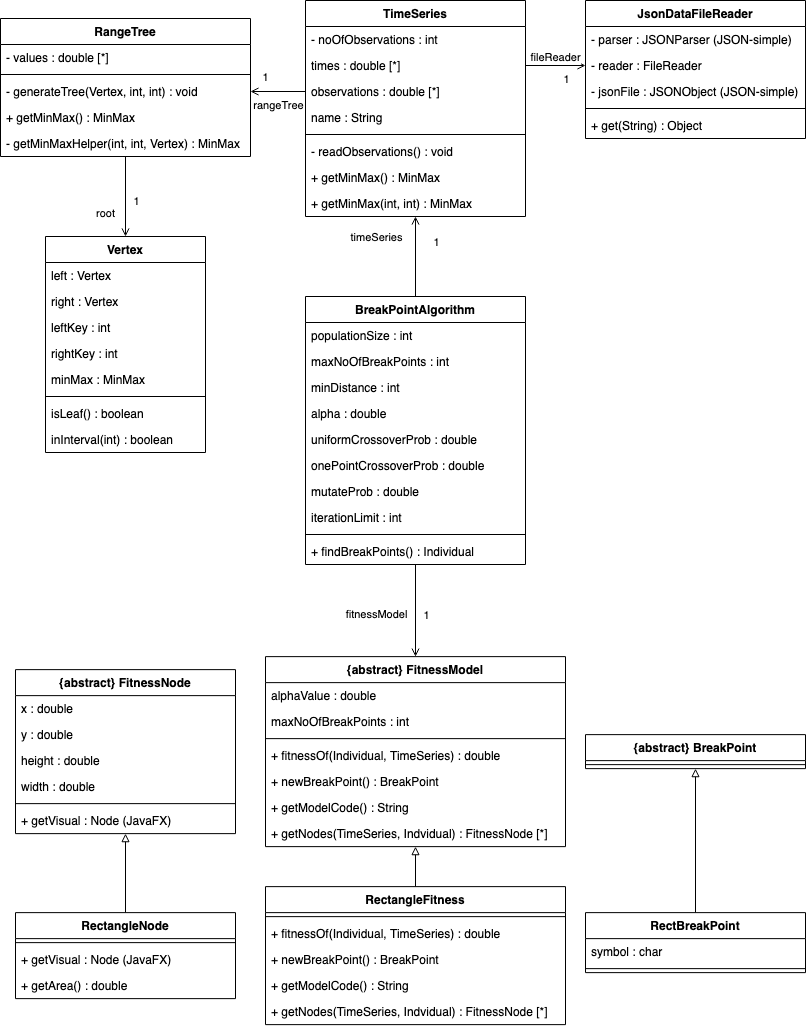
\includegraphics[width=.7\textwidth]{fig/class-diagram-algorithm.png}
    \caption{Class diagram of the break point algorithm with time series and fitness}
    \label{fig:class-diagram-algorithm}
\end{figure}

\clearpage
\section{Optimized range tree query algorithm example} \label{app:range-tree-query}

A few scenarios can
occur. These scenarios will be illustrated by calling the query range $[1,5]$ on
the tree in figure~\ref{fig:range-tree-ex}. 

\begin{itemize}
    \item In the beginning, the two paths can follow each other. This is the
    case since the left child has the range $[0,7]$ and $0 < 1 < 5 < 7$. The
    algorithm goes into the left child node and the query range remains $[1,5]$. 

    \item At the left child node, the two paths must split since $1 \in [0,3]$
    and $5 \in [4,7]$. 

    During the split up, two things will happen: The algorithm will go into both
    children respectively \textit{and} the query range going into the either
    child will be \textit{updated}.

    Going into the left child, the query range is updated to $[1,3]$. Notice
    that the lower bound remains the same but the upper bound is
    updated. This is because, for all children of the node with range $[0,3]$,
    the upper bound cannot exceed $3$. 

    Going into the right child, the query range is updated to $[4,5]$. Here, the
    upper bound stays the same, but the lower bound is updated to $4$. Again,
    this is because, in this side of the tree, no children can have a lower
    bound $< 4$. 

    At the end, the algorithm combines the query result of the left and the
    right path. 

    \item Now the left path (with query range $[1,3]$ is at the node with range
    $[0,3]$. The lower bound $1$ is the left child but the upper bound $3$ is in
    the right child. Now, the algorithm once again splits up. But notice that,
    going into the right child, the query range is updated to $[2,3]$. This is
    exactly the range of that node, so the result from that node is returned.
    For the left path, this will always be case for when the path is "splitting
    up": The query range going into the right child will be equal to the range
    of the right child and the algorithm stops here and returns that nodes
    minimum and maximum. 

    The left path continues into the node with range $[0,1]$ with range query
    $[1,1]$. This makes the path go into the right child where it returns the
    minimum and maximum value from that node given it is a leaf. 

    \item From the split, the right path (with query range $4,5$) goes into the
    node with range $[4,7]$. Given that $5 \in [4,5]$ the path goes to the left
    child with query range remaining as $[4,5]$. Notice that the left child also
    has the range $[4,5]$ and the path then ends here and returns the result. 

\end{itemize}

\begin{figure}[ht]
    \centering
    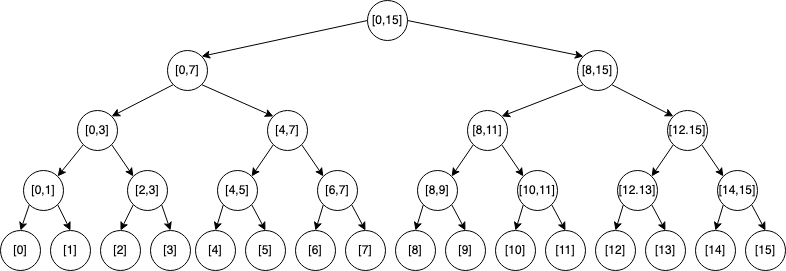
\includegraphics[width=.8\textwidth]{fig/range-tree-ex.png}
    \caption{Example of a range tree with ranges. }
    \label{fig:range-tree-ex}
\end{figure}